%% LaTeX-Beamer template for KIT design
%% by Erik Burger, Christian Hammer
%% title picture by Klaus Krogmann
%%
%% version 2.1
%%
%% mostly compatible to KIT corporate design v2.0
%% http://intranet.kit.edu/gestaltungsrichtlinien.php
%%
%% Problems, bugs and comments to
%% burger@kit.edu

\documentclass[18pt]{beamer}
\usepackage[utf8x]{inputenc}
\usepackage{units}
\usepackage{booktabs}

%% CUSTOM
\usepackage{amsmath}
\usepackage{algpseudocode}

%% Definitions
\DeclareMathOperator{\div2}{div}
\renewcommand{\algorithmicrequire}{\textbf{Input:}}
\renewcommand{\algorithmicensure}{\textbf{Output:}}
\algnewcommand\algorithmicto{\textbf{to}}
\algrenewtext{For}[3]{\algorithmicfor\ $#1 \gets #2$ \algorithmicto\ $#3$ \algorithmicdo}
\algnewcommand\algorithmicod{\textbf{od}}
\algrenewtext{EndWhile}{\algorithmicod}
\algrenewtext{EndFor}{\algorithmicod}
%\AtBeginSection[]{%
%\begin{frame}<beamer> % do nothing in handouts
%    \frametitle{Überblick}
%    \tableofcontents[sectionstyle=show/shaded,
%    subsectionstyle=show/show/hide]
%\end{frame}
%}
%\AtBeginSubsection[]{%
%\begin{frame}<beamer> % do nothing in handouts
%    \frametitle{Überblick}
%    \tableofcontents[sectionstyle=show/shaded,
%    subsectionstyle=show/shaded/hide]
%\end{frame}
%}

%% SLIDE FORMAT

% use 'beamerthemekit' for standard 4:3 ratio
% for widescreen slides (16:9), use 'beamerthemekitwide'

\usepackage{templates/beamerthemekit}
%\usepackage{templates/beamerthemekitwide}

 %% TITLE PICTURE

 % if a custom picture is to be used on the title page, copy it into the 'logos'
 % directory, in the line below, replace 'mypicture' with the 
 % filename (without extension) and uncomment the following line
 % (picture proportions: 63 : 20 for standard, 169 : 40 for wide
 % *.eps format if you use latex+dvips+ps2pdf, 
 % *.jpg/*.png/*.pdf if you use pdflatex)


 \titleimage{banner}
 
 
%% Define some colors:
\definecolor{darkblue}{rgb}{0,0,.5}
\definecolor{darkgreen}{rgb}{0,.5,0}

 %% TITLE LOGO

 % for a custom logo on the front page, copy your file into the 'logos'
 % directory, insert the filename in the line below and uncomment it

\titlelogo{logo_150x150}
 
 % (*.eps format if you use latex+dvips+ps2pdf,
 % *.jpg/*.png/*.pdf if you use pdflatex)
 
 %% TikZ INTEGRATION
 
 % use these packages for PCM symbols and UML classes
 % \usepackage{templates/tikzkit}
 % \usepackage{templates/tikzuml}
 
 % the presentation starts here
 
\author{Dominik Muth - dominik.muth@student.kit.edu}
\institute{Institut f\"ur Informatik}


\title[Tutorium 7]{GBI Tutorium Nr. $2^5$}
\subtitle{Tutorium 7}
\date{5. Dezember 2012}

% Bibliography



\begin{document}

	%title page
	\begin{frame}
		\titlepage
	\end{frame}

	%table of contents
	\begin{frame}{Outline/Gliederung}
		\tableofcontents
	\end{frame}
	
	
	
	\section{\"Ubungsblatt 6}
	\begin{frame} {Übungsblatt 6}
		\begin{block}{Aufgabe 6.2)}
			Gegeben seien die beiden Abbildungen 
			$f: X \rightarrow Y$ und $g: Y \rightarrow Z$. Zeigen Sie:
			\begin{itemize}
				\item $f$ und $g$ sind injektiv 
				$\Rightarrow g \circ f$ ist injektiv.
				\item $f$ ist nicht surjektiv und $g$ ist injektiv 
				$\Rightarrow g \circ f$ ist nicht surjektiv.
			\end{itemize}
		\end{block}
	\end{frame}	
		
	
	
	
	\section{Wiederholung} 
	\begin{frame} {Wiederholung - Quiz}
		\begin{itemize}
			\item Ein Huffman -Baum ist eindeutig 
			\only<2-> {\color{red}$X$}\\
			\color{black}
					
			\item $f(x) = 42x$ ist ein Homomorphismus
			\only<3-> {\color{darkgreen}$\surd$}\\
			\color{black}
	
			\item $Num_{-3}$ existiert nicht
			\only<4-> {\color{red}$X$}\\
			\color{black}
			
			\item Der Nikolaus verschenkt Punkte
			\only<5-> {\color{darkgreen}$\surd$\color{red}$X$}\\
			\color{black}
		\end{itemize}
	\end{frame}
	
	
	
	\begin{frame} {Wiederholung - Aufgaben}
		\begin{block}{Zahlensysteme}
			Gegeben seien folgende Definitionen: \\
			$Num_{-3}(0)=0$, $Num_{-3}(1)=-1$, $Num_{-3}(2)=-2$.\\
			Berechnen Sie folgende Werte:\\
			\begin{itemize}
				\item $Num_{-3}(\epsilon) = $\visible<2->{$\;0$}\\
				\item $Num_{-3}(201) = $\visible<3->{$\;-19$}\\
				\item $Num_{-3}(1222) = $\visible<4->{$\;13$}
			\end{itemize}			 
		\end{block}
	\end{frame}
	
	
	
	\begin{frame} {Wiederholung}
		\begin{block}{Huffman-Codierung}
			Gegeben seien folgende absolute Häufigkeiten:\\
			\vspace{5pt}
			\begin{tabular}{l||cccc}
				Häufigkeit 	& 1 & 3 & 5 & 6\\
				Zeichen		& c & b & d & a\\
			\end{tabular}\\
			\vspace{5pt}
			Decodieren sie folgendes Wort:\\
			\vspace{10pt}
			$111010111011000101101111100111$\\
			 \vspace{20pt}
			Achten sie beim aufstellen des Huffman-Baumes auf folgendes:\\
			 - sortieren Sie die Elemente aufsteigend nach ihrer Häufigkeit.\\
			 - beschriften Sie Kanten nach rechts mit 1.
			
		\end{block}
	\end{frame}
	
	
	\section{Graphen}
	\subsection{gerichtete Graphen}
	\begin{frame}{gerichtete Graphen}
		\begin{block}{Erläuterung}
			\begin{itemize}
				\item Was sind Graphen?\\
					- Knoten verbunden mit Kanten
				
				\item Wofür sind sie da?\\
					- Um Strukturen/Beziehungen darzustellen\\
					- Zum darstellen von Methoden\\
					- ...
			\end{itemize}			 
		\end{block}
	\end{frame}
	
	
	\begin{frame}{gerichtete Graphen}
		\begin{block}{Darstellung}
			Da ein Graph aus Knoten und Kanten besteht, kann man folgendes schreiben:\\
			$G = ( V, E )$\\
			Mit V = vertex = Knoten\\
			und E = edges = Kanten\\
			wobei $E \subseteq V \times V$\\
			\vspace{10pt}
			Wenn $(x,y) \in E \Rightarrow$ es existiert eine gerichtete Kante von x nach y.
		\end{block}
	\end{frame}
	
	
	\begin{frame}{gerichtete Graphen}
		\begin{exampleblock}{Beispiel}
			$ V = \{0, 1, 2, 3\}$ und $E = \{(0,1), (3,2), (2,1), (2,2)\}$
		\end{exampleblock}
		
		\begin{block}{Vorstellung}
			\begin{itemize}
				\pause
				\item Wie könnte man sich ein Einbahnstraßensystem aufzeichnen?

				\pause
				\item Wie lässt sich das auf Zweibahnstraßen übertragen?
				
				\pause
				\item und eine Autobahn?
			\end{itemize}
			
		\end{block}
	\end{frame}
	
	
	\begin{frame}{gerichtete Graphen}
		\begin{block}{Pfade und Erreichbarkeit}
			Als $Pfad$ definieren wir einen Weg von einem Knoten zu einem Anderen.\\
			\vspace{5pt}
			Ein Knoten y is genau dann von einem anderen Knoten x erreichbar, 
			wenn es einen Pfad von x nach y gibt.
		\end{block}
		
		\pause
		\begin{block}{Zyklen}
			Wenn es einen Pfad von einem Knoten x nach einem Knoten y gibt, und auch einen Pfad von y nach x, dann sprechen wir von einem Zyklus.
		\end{block}
		
		\pause
		\begin{block}{Schlingen}
			Eine Schlinge ist eine Kante von einem Knoten zu sich selbst.
		\end{block}
	\end{frame}
	
	
	\begin{frame}{Aufgabe}
		\begin{block}{}
			Gegeben sei folgender Graph:\\
			$G=(\{0,1,2,3,4,5\}, \{(1,0), (1,2), (2,3), (3,2), (3,4), (5,4), (4,0)\})$\\
			\vspace{10pt}
			\begin{itemize}
				\pause
				\item Zeichnen Sie den Graphen G
				
				\pause
				\item existiert ein Pfad von Knoten 1 zu Knoten 5?
				
				\pause
				\item Ist der Knoten 0 von allen anderen Knoten aus Erreichbar?
			\end{itemize}
		\end{block}
	\end{frame}
	
	


	\subsection{ungerichtete Graphen}
	\begin{frame}{ungerichtete Graphen}
		\begin{block}{Eigenschaften}
			Ähnlich wie bei gerichteten Graphen, nur gilt hier:\\
			Wenn $(x,y) \in E \Rightarrow$ es existiert eine ungerichtete Kante zwischen x und y.
			$\Rightarrow(x,y) = (y,x)$\\
		\end{block}
		
		\pause
		\begin{exampleblock}{Beispiel}
			$ V = \{0, 1, 2, 3\}$ und $E = \{(0,1), (3,2), (2,1), (2,2)\}$
		\end{exampleblock}
		
		\pause
		\begin{alertblock}{Achtung}
			''Einbahnstraßen" gibt es in ungerichteten Graphen nicht.
		\end{alertblock}
	\end{frame}
	
	
	\begin{frame}{Aufgabe}
		\begin{itemize}
			\item Was muss gelten, damit ein Knoten von jedem anderen Knoten aus erreichbar ist?
		
			\pause
			\item Zeichnen Sie den Graphen $G=(\{0,1,2,3\}, \{(0,1), (1,2), (2,0)\})$
		
			\pause
			\item Wie viele Kanten kann der Graph $G_4$ mit maximal vielen Kante haben?
		
			\pause
			\item Zeichnen sie den  Graph $G_4$ ohne sich überschneidende Kanten.
		\end{itemize}
	
	\end{frame}
	
	
	
	\begin{frame}{Allgemeine Eigenschaften}
		 \begin{block}{Teilgraphen}
			Ein Teilgraph G' von einem Graphen G hat folgende Eigenschaften:\\
			$V' \subseteq V$ und $E' \subseteq E'$\\
			Außerdem muss für jede Kante aus E' gelten, dass deren zwei Knoten im Teilgraph enthalten sind.
		 \end{block}
		 
		 \begin{exampleblock}{Beispiel}
		 	siehe Tafel
		 \end{exampleblock}
	\end{frame}
	
	
	\begin{frame}{Allgemeine Eigenschaften}
		 \begin{block}{Isomorphie}
		 	Graphen sind Isomorph, falls sie bis auf die Benennung der Knoten gleich sind.\\
		 	\vspace{5pt}
		 	Einen Isomorphismus kann man als Tabelle darstellen, Beispiel folgt
		 \end{block}
		 
		 \begin{exampleblock}{Beispiel}
		 	Geben Sie den Isomorphismus zwischen:\\
		 		$G_1 = (\{1,2,3,4\}, \{(1,2),(2,3),(3,4)\})$ und\\
		 		$G_1 = (\{a,b,c,d\}, \{(a,c),(c,b),(b,d)\})$
		 \end{exampleblock}
	\end{frame}
	
	
	
	\begin{frame}{Aufgabe}
		Für welche der folgenden sechs Graphen gibt es einen
    	Isomorphismus zu einem der anderen fünf Graphen? Geben Sie jeweils
    	den zugehörigen Isomorphismus an.

		\begin{center}
			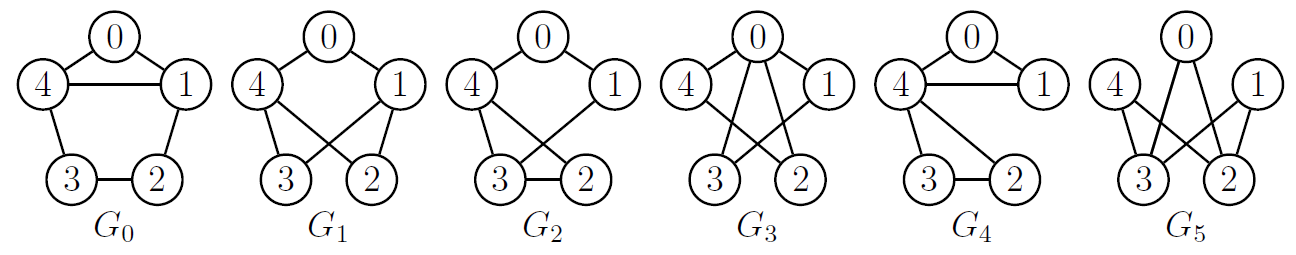
\includegraphics[scale=0.3]{graphics/07/isomorphie.png}
		\end{center}
   
	\end{frame}
	
	
	\subsection{Bäume}
	\begin{frame}{Bäume}
		\begin{block}{Definition}
			Bäume sind Spezielle Graphen mit besonderen Eigenschaften:\\
			\begin{itemize}
				\item G ist zusammenhängend
				\item $|E| = |V| - 1$
				\item G ist zyklenfrei
				\item G ist Schlingenfrei
			\end{itemize}
		\end{block}
	\end{frame}
	
	
	\begin{frame}{Aufgabe}
		Beweisen Sie: Ein ungerichteter Graph $G = (V,E)$ ist ein Baum $\Leftrightarrow (|V| =
|E| + 1$ und G hat keine Zyklen).
	\end{frame}
	
	
	
	\subsection{Graphen mit Markierungen}
	\begin{frame}{Graphen mit Markierungen}
		\begin{block}{kantenmarkierte Graphen}
			Wozu?\\
			\begin{itemize}
				\pause
				\item Codierung (siehe Huffman Baum)
				\pause
				\item ...
			\end{itemize}
		\end{block}
		
		\pause
		\begin{block}{Graphen mit gewichteten Kanten}
			Kanten werden mit Werten versetzt.\\
			Wozu?\\
			\begin{itemize}
				\pause
				\item für Entfernungen (z.B. Navigation)
				\pause
				\item für Auslastungen (z.B. Internet)
				\pause
				\item für Zeit (z.B. Zeitplanung)
				\item ...
			\end{itemize}
		\end{block}
	\end{frame}
	
	
	\begin{frame}{Aufgaben}
		\begin{block}{Wege}
			Gegeben sei folgender Graph:\\
			\begin{center}
				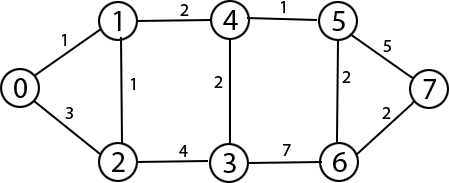
\includegraphics[scale=0.5]{graphics/07/graph.png}
			\end{center}
			
			\begin{itemize}
				\item Geben Sie den Kürzesten möglichen Weg von 0 nach 7 an.
				\item Geben Sie den längsten möglichen Weg von 0 nach 7 an.
			\end{itemize}
			*Hinweis, jeder Knoten darf maximal 1 mal durchlaufen werden.
		\end{block}
	\end{frame}
	
	
	
	\begin{frame}{Aufgaben}
		\begin{block} {ÜB7 (WS08/09)}
			Gegeben sei der Graph $G = (V,E)$ mit $V = \{0,1\}^3$ und $E = \{(xw, wy)\;|\;x,< \in \{0,1\} \land w \in \{0,1\}^2\}$.
			
			\begin{itemize}
				\item Zeichen Sie den Graphen
				\item Geben Sie einen Zyklus in G an, der außer dem 
					Anfangs- und Endknoten jeden Knoten von G genau einmal enthält.
				\item Geben Sie einen geschlossenen Pfad in G an, 
					der jede Kante von G genau einmal enthält.
			\end{itemize}
		\end{block}
	\end{frame}
	
	
	
	
	\section{Fragen}
	\begin{frame} {Fragen}
		\begin{itemize}
			\item Fragen zum Stoff?
			\item Fragen zum n\"achsten \"Ubungsblatt?
			\item Generelle Fragen?
			\item Feedback?
		\end{itemize}
	\end{frame}

		
	\begin{frame} {EOF}
		\begin{center}
			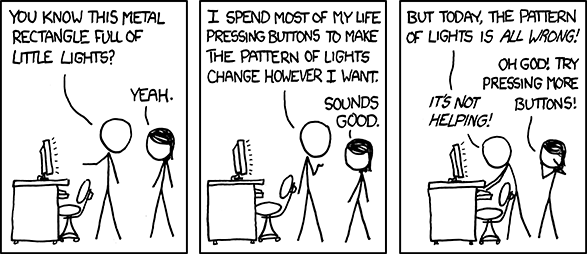
\includegraphics[scale=0.6]{graphics/eof7.png}\\
			\tiny $source: http://imgs.xkcd.com/comics/computer\_problems.png$
		\end{center}
	\end{frame}

\end{document}
